\section{Valuation}
Valuation of options has been a great area of research, starting with Black-Scholes derivatives pricing and building upon it.
    Relevant for accounting statements and tax returns - FASB has changed valuation practices several times to ensure harmonization
    shape of valuation function → executive's exposure to risk and incentives
    valuation and hedge ratio/delta provide approximation of the incentive of option (which remain however limited and dependent on the full comp package!)

    %Objective value: use binomial model mainly
    %Subjective value: certainty equivalence procedure

    %Note that in the below we assume that the stock price follows a simple geometric Brownian motion, not influenced by the agents' actions, which is standard in the literature. A different approach could be accounting for it, at least in the executive valuation part, which could be a sensible thing to do. Anyhow, our approach can be seen as a lower bound approximation for such revised executive value (with effort = 0 and no additional executive-induced volatility).


\subsection{Valuation models} 

\subsubsection*{Black-Scholes}
    The Black-Scholes model, developed by Fischer Black and Myron Scholes in the early 1970s (\cite{black1973pricing}), is a well-known mathematical framework used in finance to determine the theoretical value of European-style options. A more detailed overview of the model is out of our scope and can be easily found online. We will just limit ourselves to the minimum requirements and intuition to be able to use the Black-Scholes model in computing the time-value of our ESOs later.
    
    The assumptions are quite standard, so we simply take them from \cite{wiki:blackscholes}:

    \begin{assumption}
        \label{ass:bs_1}
        The rate of return on the riskless asset is constant and denoted as risk-free interest rate $r$.
    \end{assumption}
    

    \begin{assumption}
        \label{ass: bs_2}
        The instantaneous log return of the stock price is an infinitesimal random walk with drift: the stock price follows a geometric Brownian motion, and it is assumed that the drift and volatility of the motion are constant.
    \end{assumption}

    \begin{assumption}
        \label{ass:bs_3}
        The stock does not pay any dividends.
    \end{assumption}

    \begin{assumption}
        \label{ass:bs_4}
        The market is arbitrage-free.
    \end{assumption}

    \begin{assumption}
        \label{ass:bs_5}
        It is possible to borrow and lend any amount (even fractional) of cash at the riskless rate.
    \end{assumption}

    \begin{assumption}
        \label{ass:bs_6}
        It is possible to buy and sell any amount (even fractional) of the stock.
    \end{assumption}
    
    \begin{assumption}
        \label{ass:bs_7}
        There are no transaction fees.
    \end{assumption}
    
    Note that the first three assumptions are about the underlying asset while the last four are about the market. Moreover, the penultimate assumption assumes the possibility of short-selling, which in the case of ESOs is usually not feasible. However, the Black-Scholes model provides nevertheless a good approximation and suffices for our (limited) use. Note however that not all of these assumptions are strictly necessary: extensions of this basic model are able to account for dynamic interest rates, transaction costs and taxes, and dividend payout.  

    Under these assumptions, \cite{black1973pricing} showed that it is possible to create a hedged position (i.e., a long position in the underlying stock and a long position in the option) whose value is independent of the price of the underlying. This dynamic hedging strategy leads to a partial differential equation governing the price of the option, whose solution is given by the Black-Scholes formula.

    However, despite its mathematical rigor and closed-form solution, as well as computational efficiency, the Black-Scholes can only be used with European options (options exercisable only at maturity). Therefore, since we are dealing with American ESOs, we need to resort to a different valuation methodology: binomial model.

\subsubsection*{Binomial Model} 
The binomial model was first proposed by William Sharpe in the 1978 (\cite{sharpe1978investments}) and later formalized by Cox, Ross and Rubinstein (CRR) in 1979 (\cite{cox1979option}). It uses a lattice-based approach to model the price of the underlying stock price. We employ it to value our executive stock options, since they are, as we saw before, American option.\footnote{Recall that Black-Scholes can be used only with European options, i.e., options exercisable only at maturity. Nevertheless, Black-Scholes valuation provides a lower-bound to the value of American options. Indeed, giving the holder the possibility to exercise before maturity also cannot be worse for her, because she can always simply hold the option up to maturity and then deciding, mimicking thus a European option.}
Similarly to Monte Carlo simulations and finite difference methods, the binomial options pricing model does not yield a closed-form solution, but works quite well with sufficiently high number $n$ of time steps, i.e., with a sufficiently discretized grid (i.e., a small $\Delta t$). Clearly, for European options, as $\Delta t \rightarrow 0$, the binomial model approaches the Black-Scholes value.

We need the assumptions \ref*{ass:bs_1}, \ref*{ass:bs_3}, \ref*{ass:bs_4}, \ref*{ass:bs_7} from Black-Scholes, and in addition we pose two additional assumptions:

\begin{assumption}
    \label{ass:bin_8}
    Time is divided into discrete periods.
\end{assumption}

\begin{assumption}
    \label{ass:bin_9}
    At any time step, the underlying's price can only move one of two ways: either up or down.
\end{assumption}

The intuition behind the model is quite simple. We discretize the evolution of the underlying stock price by building a binomial lattice (tree), for a given number of steps between the issue of the option and its maturity. Each node represents thus a possible price of the underlying stock. From each node, the stock price can either go up ($u$) or down ($d$). The key assumption is thus that the stock moves only in either one of these two directions. Therefore, the generic value of the stock at step $t$ with $k$ upward movements and $t-k$ downward movements is $S_t = S_0 u^k d^{t-k}$, where $S_0$ is the initial stock price at $t=0$. Figure \ref*{fig:bin_tree} provides a graphical representation of the first two levels of the stock price tree. 

\vspace*{3pt}
\begin{figure}[!h]
\vspace*{10pt}
\centering
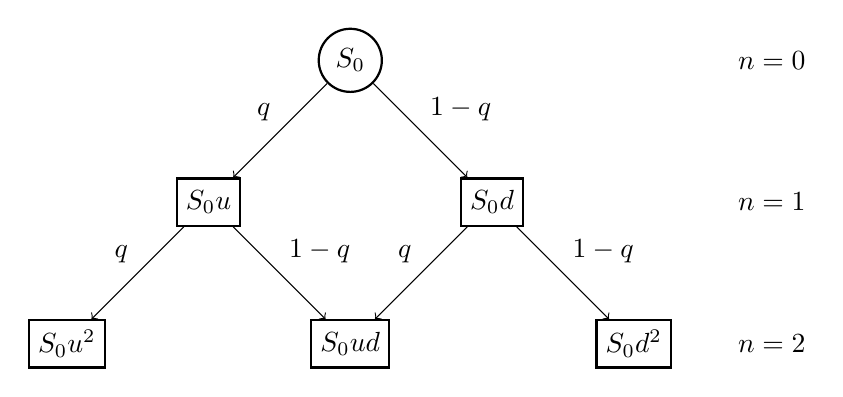
\begin{tikzpicture}[
    roundnode/.style={circle, draw=black, thick, minimum size=6mm},
    squarednode/.style={rectangle, draw=black, thick, minimum size=6mm},
    scale=1.2
  ]
  
  %Nodes
  \node[roundnode] at (0,0) (A) {$S_0$};
  \node[squarednode] at (-1.5,-1.5) (B) {$S_0 u$};
  \node[squarednode] at (1.5,-1.5) (C) {$S_0 d$};
  \node[squarednode] at (-3,-3) (D) {$S_0 u^2$};
  \node[squarednode] at (0,-3) (E) {$S_0 ud$};
  \node[squarednode] at (3,-3) (F) {$S_0 d^2$};  
  
  %Lines
  \draw[->] (A) -- (B) node[midway,above left] {$q$};
  \draw[->] (A) -- (C) node[midway,above right] {$1-q$};
  \draw[->] (B) -- (D) node[midway,above left] {$q$};
  \draw[->] (B) -- (E) node[midway,above right] {$1-q$};
  \draw[->] (C) -- (E) node[midway,above left] {$q$};
  \draw[->] (C) -- (F) node[midway,above right] {$1-q$};
  
  %Labels
  \node[right] at (4,0) {$n=0$};
  \node[right] at (4,-1.5) {$n=1$};
  \node[right] at (4,-3) {$n=2$};

\end{tikzpicture}
\caption{Representation of the binomial tree with n=2} 
\label{fig:bin_tree}
\end{figure}
\newpage  %%-> FIX q/1-q location on arrows

We can divide the procedure in three main steps: (i) build the stock tree, (ii) calculate the option value at each terminal node, (iii) go backwards and decide at each node whether it is optimal to exercise or keep the option.

We use the original CRR method and set $u = e^{\sigma \sqrt{\Delta t}}$ and $d = e^{-\sigma \sqrt{\Delta t}}=\frac{1}{u}$, which are the multiplicative factors if the stock price goes up or down, respectively. Therefore, the value of the stock when it goes up or down depends also on its underlying volatility. Moreover, the condition $d = \frac{1}{u}$ ensures that the tree is recombinant, meaning that what matters is the number of ups and downs, not their order. This means that if the stock price moves up and then down, the stock price will be the same as if it instead moved first down and then up. This is convenient also because it allows the tree representation of the underlying stock price, ensuring that all the nodes are nicely connected, and it fastens the calculation of the option price (indeed, note that in this way the number of total nodes is reduced). 

In the second step, we simply compute the option value at expiration, i.e., its intrinsic value, which in our case is $\max \{0, S_T - K \}$ since we have a call option.

For the third step, we need to introduce the risk-neutral probability $q = \frac{e^{-r \Delta t} - d}{u-d}$ which assesses how likely is that the stock price goes up during each period in a risk-neutral world. \footnote{This choice of $q$ allows for the related binomial distribution to simulate the geometric Brownian motion of the underlying stock, with parameters $r$ and $\sigma$.} In this world, today's fair price of the option is the expected value of its future payoff discounted by the risk-free rate. Therefore, the expected value at time $t$ is calculated using the option values from the subsequent two nodes at $t+1$, weighted by their respective probabilities - $q$ as the probability of an upward move of the underlying stock, $1-q$ of a downward move. This value is then discounted using $r$ and represents the \textit{binomial value} of the option at a given node. 
Given $q$, we can then proceed with our backwards algorithm. We start at each pre-terminal node and evaluate whether it is optimal to exercise (with payoff the stock price at the node minus the strike price) or to not exercise (with payoff the binomial value at the node). We continue this process iteratively going backwards until when the option is vested. When the option is not vested anymore, the holder cannot exercise it and so the value of the option will simply be the binomial value, at that node and all the previous ones.
The value of the option at the initial node, obtained with this backwards procedure, is the value of the ESO we obtain using the binomial model.

\subsection{Firm cost} 
%Objective value

We compute the cost of the two options to the firm using the classical valuation standards for ESOs: a simple binomial model for the RN option, and a modified binomial model that accounts for the recovered time premium for the R option.
Recall indeed that the theoretical value of an option at any time $t$ is given by (i) the intrinsic value ($S_t - K$) and (ii) the time premium, i.e., the remaining value forfeited at exercise, as the option could have appreciated in the remaining lifetime. 
We employ the \cite{cox1979option} initial binomial tree approach; however, we account for "deterministic" early exercise introducing a threshold above which the holder will exercise, i.e., always exercise if $S_t \ge Km$ for some multiple m (\dots).

We now comment the relevant code used - the full code can be found in the appendix.

\subsubsection*{RN option}
The function rn\_eso is defined as \verb|rn_eso(S0,K,T,v,r,N,sigma,m)| and takes the following parameters as input:
\begin{itemize}
    \item $S$: spot price of the underlying firm stock
    \item $K$: strike price of the option. In our case, we always set it equal to S (fn: some propose to set it slightly higher ...)
    \item $T$: time to maturity (in years)
    \item $v$: vesting period of the option (in years)
    \item $r$: risk-free interest rate
    \item $N$: height of the tree
    \item $sigma$: volatility of the underlying firm stock
    \item $m$: exercise multiple
\end{itemize}
    
 As illustrated before, we first construct the stock price tree and then compute backwards the option's value. At each step, the relevant decision is the following: if the option is either not vested or is vested but is not above the threshold for early exercise, the value at the node is the binomial value. Otherwise, if it is vested and above the threshold for early exercise, the value at the node is the exercise value. This is illustrated in the snippet below.

 \begin{lstlisting}[breaklines, basicstyle=\ttfamily\small]
    if not vested: 
        C[j] = disc * (q*C[j+1] + (1-q)*C[j])
    elif vested & (S>=K*m):            
        C[j] = S - K
    elif vested & (S<K*m):
        C[j] = disc * (q*C[j+1] + (1-q)*C[j])
 \end{lstlisting}



\subsubsection*{R option}
We define the function r\_eso as:

\begin{lstlisting}[breaklines, basicstyle=\ttfamily\small]
    r_eso(S0,K,T,v,r,N,sigma,m,alpha,gamma)
\end{lstlisting}


Apart from the parameters used before, we also need:
\begin{itemize}
    \item $\alpha$: amount of option that gets converted to stock at exercise
    \item $\gamma$: \textit{risk premium} granted in terms of new RN option 
\end{itemize}


\cite{huang2013dynamic} propose the following for their model, which we can interpret as $\gamma = 0$. 
When exercising, the payoff is given not only by the difference between stock price and exercise price, but also by the time value that gets recouped.

time value = option's full value, given by BS, MINUS the exercise value

They use Black-Scholes to account for the remaining time-value of the option at exercise. 
\begin{lstlisting}[breaklines, basicstyle=\ttfamily\small]
    if not vested:                
        C[j] = disc * (q*C[j+1] + (1-q)*C[j])
    elif vested & (S >= K*m): 
        C[j] = S - K + (1-alpha+gamma)*(black_scholes(S,K,T,r,sigma)-(S-K))
    elif vested & (S < K*m):
        C[j] = disc * (q*C[j+1] + (1-q)*C[j])
 \end{lstlisting}


% I propose the following modification to this, since the premium $\gamma$ is not properly intrinsic value.
% \begin{lstlisting}[breaklines, basicstyle=\ttfamily\small]
%     if not vested:                         
%         C[j] = disc * (q*C[j+1] + (1-q)*C[j])
%     elif vested & (S >= K*m):                
%         C[j] = S - K + (1-alpha)*(black_scholes(S,K,T,r,sigma)-(S-K)) + gamma*rn_eso(S,S,T,v,r,N,sigma,m)
%     elif vested & (S < K*m):  
%         C[j] = disc * (q*C[j+1] + (1-q)*C[j])
%  \end{lstlisting}



Using their same inputs (...), we obtain their same results. However, this is true only when 

%Show table with simulations at different n
%Simulate also with trinomial model




\subsection{Executive value}
%Subjective value

%Build up on previous code
%%% Can re-use the stock price movements (both binomial and trinomial ways)
%%% Calculate at each node the utility from max{exercise, do NOT exercise}
%%%%%% -> find the utility value at initial node through recursion
%%% Using the inverse of the utility function, find the cash level that yields the same utility

%%% NOTE that our methodology is different from simply taking the value of the option computed before at the initial node and plugging it in.

Idea: find $E_c$ so that $U(n, c) = U(0, E_c)$

Forward Shooting Grid is basically an extension of 

We re-use some notions from above, since we still use a lattice based model and mimic the idea of solving backwards.
We use \cite{lau2005valuation} approach with FSG, which is basically an extended model of the binomial model, where we also keep a vector of auxiliary variables that influece the executive's choice at each node. 




\subsection{Comparative statics}
%Simulations to compare the two values

%Deadweight loss: (cost - value)/cost * 100%


* effect of time vesting?? "time vesting has a relatively small impact on valuation but may dramatically affect the optimal exercise policy" \cite{dybvig2003employee}

